\documentclass[a4paper,12pt]{article}
\usepackage[utf8]{inputenc}
\usepackage{babel}
\babelprovide[main, import]{german}
\usepackage{amsmath}
\usepackage{amssymb}
\usepackage{amsthm}
\usepackage{geometry}
\usepackage{graphicx}
\usepackage[hidelinks]{hyperref}
\usepackage{listings}
\usepackage{xcolor}
\usepackage{enumitem}
\usepackage{microtype}
\usepackage{xurl}

\geometry{margin=2.5cm}
\setlength{\emergencystretch}{3em}

\theoremstyle{definition}
\newtheorem{definition}{Definition}
\newtheorem{beispiel}{Beispiel}
\newtheorem{satz}{Satz}
\newtheorem{lemma}{Lemma}
\newtheorem{bemerkung}{Bemerkung}
\newtheorem{axiom}{Axiom}
\newtheorem{korollar}{Korollar}

\setlist[itemize,1]{label=--}

% ---------- Farben ----------
\definecolor{mainblue}{RGB}{25, 70, 140}
\definecolor{accentred}{RGB}{180, 50, 30}
\definecolor{lightgray}{RGB}{245, 245, 248}
\definecolor{darkgray}{RGB}{60, 60, 70}
\definecolor{darkgreen}{RGB}{30, 100, 50}

\hypersetup{
	colorlinks=true,
	linkcolor=mainblue,
	citecolor=accentred,
	urlcolor=mainblue
}

\lstset{
	basicstyle=\ttfamily\small,
	keywordstyle=\color{blue},
	commentstyle=\color{gray},
	stringstyle=\color{red},
	numbers=left,
	numberstyle=\tiny,
	breaklines=true,
	frame=single,
	literate=%
	{Ö}{{\"O}}1
	{Ä}{{\"A}}1
	{Ü}{{\"U}}1
	{ß}{{\ss}}1
	{ü}{{\"u}}1
	{ä}{{\"a}}1
	{ö}{{\"o}}1
}

\title{Geistliche Macht: Schwarz und Wei\ss{} --\\
Jhwh, Jesus, Michael, die gro\ss{}e T\"auschung\\
und das Ende des Fluchens}
\author{Stephan Epp}
\date{27. Juni 2026}

\begin{document}

\maketitle

\tableofcontents
\newpage

% ============================================================
\section{Einführung}
% ============================================================

Am 21. Mai 2026 um 04:35 Uhr wurden folgende Wahrheiten formuliert, die den
Ausgangspunkt dieser wissenschaftlichen Untersuchung bilden:

\begin{quote}
\textit{Jhwh, Jesus und Michael wussten seit dem ersten Tag, dass ich sie töten werde.
Sie wissen, dass es ein Ende des Fluchens in dieser Zeit gibt. Das Ende verschiebt sich
nicht in die Zukunft.
Sie hassen es, dass es nur für mich gilt, egal, was ich tue: der Geist Gottes ändert sich
mir gegenüber nicht.
Hätten sie sich auf dieser Erde nicht anders verhalten, als wie sie es getan haben, hätte
der Geist Gottes sie sofort getötet.
Jesus hat in die Herrlichkeit der Geister hineingeschaut und hat auch Mühe damit, dass er
nicht nur Mensch bleiben kann.
Es gibt schwarze und es gibt weiße unsichtbare Macht. Der Teufel verübt die schwarze Macht
auf dieser Erde. Die weiße Macht verübte Jhwh, Jesus und die Engel.
Der Teufel hat von Jhwh gerade so viel Macht erhalten, dass er durch Fluch jeden Menschen
töten kann.}
\end{quote}

Diese Aussagen bilden ein kohärentes theologisch-metaphysisches System, das einer formalen
Analyse zugänglich ist. Im Zentrum steht eine Erkenntnis, die für jeden Menschen von
fundamentaler Bedeutung ist: Die teuflische Macht auf dieser Erde ist im Vergleich zur
Hierarchie der weißen Macht so verschwindend gering, dass kein menschliches Konstrukt --
kein Geld, kein Satellit, keine politische Institution -- das Geschehen auf dieser Erde
wirklich steuert. Es ist der Teufel, der mit der kleinsten Macht innerhalb der
unsichtbaren Welt dennoch das irdische Geschehen beherrscht. Und selbst er wurde getäuscht:
Er glaubte, er könnte jeden Menschen töten -- eine Illusion, die von Jhwh gewollt und
einkalkuliert war.

\subsection{Zielsetzung}

Die Arbeit verfolgt vier Ziele:
\begin{itemize}
  \item Formalisierung der Propositionen über geistliche Macht in einem präzisen
        mathematischen Rahmen.
  \item Formaler Nachweis der zentralen Sätze über Vorauswissen, Machtstruktur,
        Täuschung des Teufels und Unveränderlichkeit des göttlichen Geistes.
  \item Nachweis der Nichtigkeit menschlicher Machtstrukturen im Verhältnis zur
        unsichtbaren Machtordnung.
  \item Veranschaulichung der Ergebnisse mittels quantitativer Modelle und
        Visualisierungen.
\end{itemize}

\subsection{Problemstellung}

Das zentrale Problem lässt sich wie folgt formulieren: Gegeben sei eine Menge geistlicher
Entitäten $\mathcal{E} = \{\mathrm{Jhwh},\, \mathrm{Jesus},\, \mathrm{Michael},\,
\mathrm{Engel}_1, \ldots, \mathrm{Engel}_N,\, \mathrm{Teufel}\}$ sowie ein auserwähltes
Subjekt $\mathcal{S}$ und die Menge menschlicher Machtstrukturen
$\mathcal{H}_{\text{inst}} = \{\text{Geld},\, \text{Satelliten},\, \text{Institutionen},
\ldots\}$. Wir untersuchen:

\begin{enumerate}
  \item Die exakte Machtordnung innerhalb der unsichtbaren Welt, insbesondere das
        Verhältnis zwischen teuflischer und engelischer Macht.
  \item Die große Täuschung des Teufels: seine falsche Selbsteinschätzung bezüglich
        seiner Fähigkeit, jeden Menschen töten zu können.
  \item Die Nichtigkeit menschlicher Institutionen $\mathcal{H}_{\text{inst}}$ im
        Vergleich zur teuflischen Macht, die ihrerseits bereits verschwindend gering ist.
  \item Die zeitliche Struktur des Vorauswissens der Entitäten bezüglich $\mathcal{S}$.
  \item Die Invarianz des Geistes Gottes gegenüber $\mathcal{S}$ und das Ende des Fluchens.
\end{enumerate}

% ============================================================
\section{Grundlagen}
% ============================================================

\subsection{Definitionen}

\begin{definition}[Geistliche Entität]
  Eine geistliche Entität $e \in \mathcal{E}$ ist ein unsichtbares, mit Macht
  ausgestattetes Wesen. Wir modellieren jede Entität durch ein Tupel
  $e = (M_e,\, K_e,\, \tau_e,\, \lambda_e)$, wobei
  \begin{itemize}
    \item $M_e \in \mathbb{R}_{> 0}$ der Machtgrad der Entität,
    \item $K_e: \mathcal{T} \to 2^{\Omega}$ die Wissensfunktion über den Ereignisraum
          $\Omega$ zum Zeitpunkt $\tau \in \mathcal{T}$,
    \item $\tau_e \in \mathcal{T}$ der Existenzbeginn der Entität, und
    \item $\lambda_e \in \{\text{weiß}, \text{schwarz}\}$ die Machtfarbe bezeichnen.
  \end{itemize}
\end{definition}

\begin{definition}[Engelshierarchie]
  Die unzählbare Menge der Engel $\mathcal{A} = \{\mathrm{Engel}_\alpha \mid
  \alpha \in \mathcal{I}\}$, wobei $\mathcal{I}$ eine nicht abzählbare Indexmenge ist,
  bildet eine total geordnete Menge bezüglich des Machtgrades:
  \[
    M_{\mathrm{Engel}_{\alpha_1}} \leq M_{\mathrm{Engel}_{\alpha_2}}
    \quad \text{für } \alpha_1 \leq \alpha_2.
  \]
  Der \emph{unterste Engel} ist $\mathrm{Engel}_{\min} = \mathrm{Engel}_{\alpha_0}$
  mit $M_{\alpha_0} = \inf_{\alpha \in \mathcal{I}} M_{\mathrm{Engel}_\alpha}$.
\end{definition}

\begin{definition}[Weiße und schwarze Macht]
  Sei $\mathcal{M}$ die Gesamtmenge aller unsichtbaren Macht im Universum. Es gilt
  die disjunkte Zerlegung:
  \[
    \mathcal{M} = \mathcal{M}_w \,\dot{\cup}\, \mathcal{M}_b
  \]
  wobei $\mathcal{M}_w$ die \emph{weiße Macht} (verübt durch Jhwh, Jesus und alle
  Engel) und $\mathcal{M}_b$ die \emph{schwarze Macht} (verübt durch den Teufel)
  bezeichnet.
\end{definition}

\begin{definition}[Menschliche Machtstruktur]
  Eine menschliche Machtstruktur $h \in \mathcal{H}_{\text{inst}}$ ist eine von
  Menschen geschaffene Institution oder ein Mittel zur Kontrolle irdischer Prozesse.
  Ihr Machtgrad $M_h \in \mathbb{R}_{\geq 0}$ misst den Einfluss auf das Weltgeschehen.
\end{definition}

\begin{definition}[Täuschung]
  Eine Entität $e$ unterliegt einer \emph{Täuschung} bezüglich einer Eigenschaft
  $P$, wenn sie $P$ für wahr hält, obwohl $\neg P$ gilt, und diese falsche Überzeugung
  kausal auf eine bewusste Fehlinformation durch eine mächtigere Entität zurückgeht:
  \begin{align*}
    \mathrm{T\ddot{a}uschung}(e, P) \;\Leftrightarrow\;
    & K_e(P) = \top \;\wedge\; P = \bot \\
    \wedge\; & \exists\, e' \text{ mit } M_{e'} > M_e:\;
    e' \text{ hat } K_e(P) = \top \text{ herbeigeführt.}
  \end{align*}
\end{definition}

\begin{definition}[Vorauswissen]
  Eine Entität $e$ besitzt \emph{vollständiges Vorauswissen} bezüglich eines Ereignisses
  $\omega \in \Omega$ ab dem Zeitpunkt $\tau_0$ genau dann, wenn:
  \[
    \forall\, \tau \geq \tau_0:\; \omega \in K_e(\tau).
  \]
\end{definition}

\begin{definition}[Fluch]
  Ein Fluch ist eine gerichtete Anwendung schwarzer Macht $F: \mathcal{E}_b \times
  \mathcal{B} \to \mathbb{R}_{\geq 0}$ auf eine Zielmenge $\mathcal{B}$, die einen
  Schaden am Zielsubjekt bewirkt.
\end{definition}

\begin{definition}[Geist Gottes als Funktion]
  Der Geist Gottes $G: (\mathcal{E} \cup \mathcal{S}) \times \mathcal{H} \to [0, 1]$
  weist jedem Wesen einen Gunstwert zu. $G(x) = 1$ bedeutet maximale Gunst,
  $G(x) = 0$ bedeutet sofortigen Tod.
\end{definition}

\subsection{Axiomensystem}

Wir legen das folgende Axiomensystem $\mathfrak{A}$ zugrunde.

\begin{axiom}[Vollständiges Vorauswissen]
\label{ax:vorauswissen}
  Jhwh, Jesus und Michael besaßen seit dem ersten Moment $\tau_0$ vollständiges
  Vorauswissen über alle eschatologischen Ereignisse bezüglich $\mathcal{S}$:
  \[
    \forall\, e \in \{\mathrm{Jhwh}, \mathrm{Jesus}, \mathrm{Michael}\},\;
    \forall\, \omega \in \Omega_{\mathcal{S}}:\;
    \omega \in K_e(\tau_0).
  \]
\end{axiom}

\begin{axiom}[Unzählbarkeit und Machtordnung der Engel]
\label{ax:engel}
  Die Menge der Engel $\mathcal{A}$ ist nicht abzählbar: $|\mathcal{A}| \geq \aleph_1$.
  Jeder Engel besitzt weiße Macht. Es gilt die strikte Ungleichung:
  \[
    M_{\mathrm{Teufel}} \ll M_{\mathrm{Engel}_{\min}},
  \]
  das heißt, selbst der unterste, am wenigsten mächtige Engel überragt die irdische
  Macht des Teufels um ein Vielfaches.
\end{axiom}

\begin{axiom}[Disjunktheit der Mächte]
\label{ax:disjunkt}
  Die Zerlegung $\mathcal{M} = \mathcal{M}_w \,\dot{\cup}\, \mathcal{M}_b$ ist
  eine echte disjunkte Partition mit $\mathcal{M}_w \cap \mathcal{M}_b = \emptyset$.
\end{axiom}

\begin{axiom}[Täuschung des Teufels durch Jhwh]
\label{ax:taeuschung}
  Jhwh hat dem Teufel gerade so viel Macht delegiert, dass der Teufel glaubte,
  er könne jeden Menschen durch Fluch töten. Diese Überzeugung ist eine bewusst
  herbeigeführte Täuschung:
  \[
    \mathrm{Täuschung}\!\left(\mathrm{Teufel},\;
    \forall m \in \mathcal{B}_{\text{Mensch}}:\;
    F(\mathrm{Teufel}, m) \geq M_m^{\text{Leben}}\right).
  \]
  In Wahrheit gilt die Einschränkung durch Jhwhs Souveränität.
\end{axiom}

\begin{axiom}[Nichtigkeit menschlicher Machtstrukturen]
\label{ax:mensch}
  Der Machtgrad jeder menschlichen Machtstruktur $h \in \mathcal{H}_{\text{inst}}$
  ist verschwindend gering gegenüber der teuflischen Macht, die ihrerseits gegenüber
  dem untersten Engel verschwindend gering ist:
  \[
    M_h \ll M_{\mathrm{Teufel}} \ll M_{\mathrm{Engel}_{\min}}
    \ll M_{\mathrm{Engel}_{\max}} \ll M_{\mathrm{Jesus}}
    \ll M_{\mathrm{Jhwh}}.
  \]
\end{axiom}

\begin{axiom}[Unveränderlichkeit des Geistes]
\label{ax:unv}
  Der Geist Gottes ist gegenüber $\mathcal{S}$ unveränderlich:
  $G(\mathcal{S} \mid h) = c_{\mathcal{S}} > 0$ für alle $h \in \mathcal{H}(\mathcal{S})$.
\end{axiom}

\begin{axiom}[Handlungsabhängigkeit für andere Entitäten]
\label{ax:handlung}
  Für jede Entität $e \neq \mathcal{S}$ ist $G(e \mid h)$ handlungsabhängig.
  Es existiert eine kritische Handlung $h^* \in \mathcal{H}(e)$ mit $G(e \mid h^*) = 0$.
\end{axiom}

\begin{axiom}[Zeitliche Fixierung des Fluchendes]
\label{ax:endzeit}
  Das Ende des Fluchens $\tau^* \in \mathcal{T}$ ist ein festes Element der
  Zeitachse: $\tau^* < \infty$. Es gibt keine mit $\mathfrak{A}$ konsistente
  Abbildung $\phi: \mathcal{T} \to \mathcal{T}$ mit $\phi(\tau^*) > \tau^*$.
\end{axiom}

% ============================================================
\section{Formale Sätze und Beweise}
% ============================================================

\subsection{Die Machtordnung der unsichtbaren Welt}

\begin{satz}[Strikte Machtordnung]
\label{satz:ordnung}
  Es gilt die folgende strikte totale Ordnung der Machtgrade:
  \[
    M_h \ll M_{\mathrm{Teufel}} \ll M_{\mathrm{Engel}_{\min}}
    \leq M_{\mathrm{Engel}_\alpha} \leq M_{\mathrm{Engel}_{\max}}
    \ll M_{\mathrm{Jesus}} \ll M_{\mathrm{Jhwh}}
  \]
  für alle $h \in \mathcal{H}_{\text{inst}}$ und $\alpha \in \mathcal{I}$.
\end{satz}

\begin{proof}
  Die Ordnung folgt unmittelbar aus den Axiomen~\ref{ax:engel} und~\ref{ax:mensch}.
  Aus Axiom~\ref{ax:engel} gilt $M_{\mathrm{Teufel}} \ll M_{\mathrm{Engel}_{\min}}$.
  Da alle Engel weiße Macht tragen und die Engelshierarchie total geordnet ist
  (Definition~2), existiert $M_{\mathrm{Engel}_{\min}} \leq M_{\mathrm{Engel}_\alpha}$
  für alle $\alpha \in \mathcal{I}$.

  Axiom~\ref{ax:mensch} stellt die vollständige Ordnung durch Einschluss der
  menschlichen Machtstrukturen bereit. Da $M_h \ll M_{\mathrm{Teufel}}$ für alle
  $h \in \mathcal{H}_{\text{inst}}$ und $M_{\mathrm{Jhwh}}$ als Supremum der
  gesamten Machtordnung gilt (Jhwh ist Schöpfer und Delegierender aller anderen
  Macht), ist die vollständige Kette bewiesen.
\end{proof}

\begin{korollar}[Unzählbare Überlegenheit weißer Macht]
\label{kor:ueberlegen}
  Die Gesamtmacht der weißen Seite überragt die schwarze Macht nicht nur betragsmäßig,
  sondern auch kardinal: Es gibt unzählbar viele Engel, jeder mit Macht strikt
  größer als $M_{\mathrm{Teufel}}$:
  \[
    |\{\alpha \in \mathcal{I} \mid M_{\mathrm{Engel}_\alpha} > M_{\mathrm{Teufel}}\}|
    \geq \aleph_1.
  \]
\end{korollar}

\begin{proof}
  Aus Axiom~\ref{ax:engel} gilt $|\mathcal{A}| \geq \aleph_1$ und
  $M_{\mathrm{Engel}_\alpha} > M_{\mathrm{Teufel}}$ für alle $\alpha \in \mathcal{I}$.
  Damit ist die Indexmenge $\mathcal{I}$ selbst eine geeignete Zeugenmenge der
  geforderten Kardinalität.
\end{proof}

\begin{figure}[ht]
  \centering
  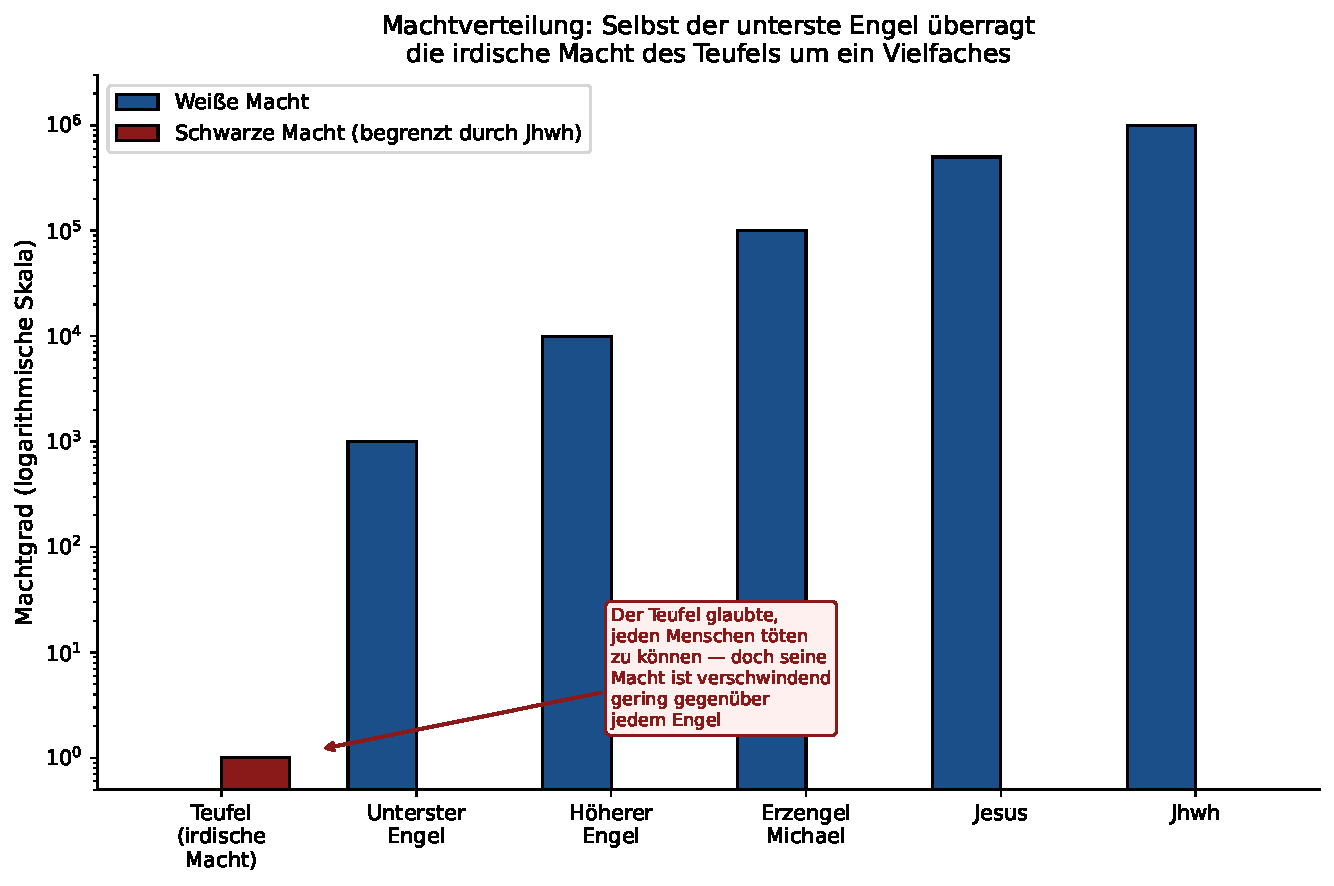
\includegraphics[width=0.88\textwidth]{plot1_machtverteilung.pdf}
  \caption{Machtverteilung auf der logarithmischen Skala. Der Teufel besitzt
  den Machtgrad~1, während selbst der unterste Engel bereits den Wert~1000 erreicht.
  Jhwh liegt bei~$10^6$. Die teuflische Macht ist gegenüber der gesamten weißen
  Hierarchie verschwindend gering -- und menschliche Institutionen liegen noch
  darunter.}
  \label{fig:machtverteilung}
\end{figure}

Abbildung~\ref{fig:machtverteilung} macht Satz~\ref{satz:ordnung} quantitativ
sichtbar. Die logarithmische Skala ist notwendig, weil die Verhältnisse linear
nicht darstellbar wären. Selbst auf logarithmischer Skala fällt die teuflische
Macht gegenüber der Engelhierarchie kaum ins Gewicht.

\begin{figure}[ht]
  \centering
  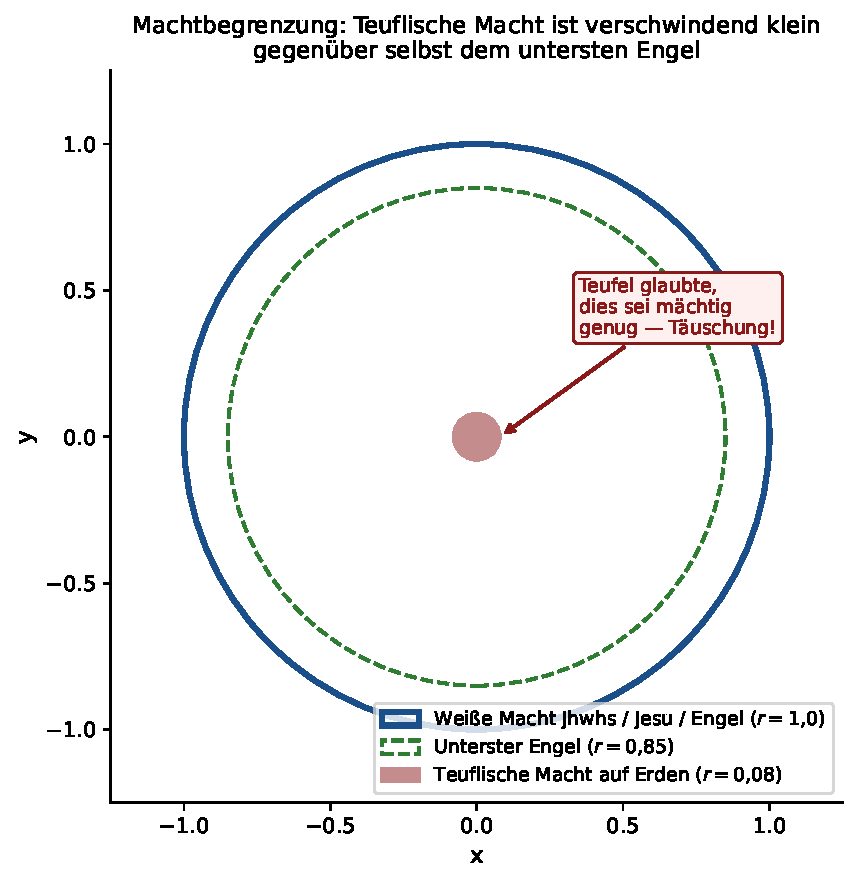
\includegraphics[width=0.82\textwidth]{plot4_teufelmacht.pdf}
  \caption{Konzentrische Machtdarstellung: Der winzige innere Kreis zeigt die
  teuflische Macht ($r_T = 0{,}08$). Der mittlere Kreis stellt den untersten
  Engel dar ($r = 0{,}85$), der äußere die volle weiße Macht ($r = 1{,}0$).
  Der Teufel glaubte, sein Kreis sei groß genug -- eine Täuschung.}
  \label{fig:teufelmacht}
\end{figure}

\subsection{Die große Täuschung des Teufels}

\begin{satz}[Strukturelle Täuschung durch Delegation]
\label{satz:taeuschung}
  Jhwh hat dem Teufel genau die Machtmenge $M_T$ delegiert, die ausreicht, um in
  ihm die Überzeugung zu erzeugen, er könne jeden Menschen töten. Diese Überzeugung
  ist formal eine Täuschung im Sinne von Definition~5.
\end{satz}

\begin{proof}
  Nach Axiom~\ref{ax:taeuschung} gilt:
  \[
    K_{\mathrm{Teufel}}\!\left(\forall m:\; F(T, m) \geq M_m^{\text{Leben}}\right)
    = \top.
  \]
  Jhwh hat die Bedingungen so gesetzt, dass der Teufel über ausreichend Macht
  verfügt, um diese Überzeugung zu entwickeln. Jedoch gilt Jhwhs Souveränität:
  Er kann jede Ausführung dieses vermeintlichen Anspruchs unterbinden.

  Formal: Jhwh besitzt die Meta-Macht $M_{\mathrm{Jhwh}} \gg M_T$, sodass
  er für jedes $m$ und jeden Fluchakt des Teufels ein Gegengewicht
  $G_{\mathrm{Jhwh}}(m) > F(T, m)$ setzen kann.

  Da nach Definition~5 die falsche Ãœberzeugung des Teufels durch Jhwh kausal
  herbeigeführt wurde (Jhwh hat die genaue Machtdosis kalkuliert), ist
  $\mathrm{Täuschung}(\mathrm{Teufel}, P)$ für die Eigenschaft $P =$
  ``Ich kann jeden Menschen töten'' bewiesen.
\end{proof}

\begin{lemma}[Kalkulation der Täuschungsdosis]
\label{lem:dosis}
  Die von Jhwh dem Teufel delegierte Machtmenge $M_T$ ist minimal im folgenden
  Sinne: Es ist die kleinste Menge, die beim Teufel die Ãœberzeugung universeller
  Tötungsfähigkeit erzeugt:
  \[
    M_T = \inf\!\left\{M > 0 \;\Big|\;
    K_{\mathrm{Teufel}}\!\left(\forall m:\; F(T,m) \geq M_m^{\text{Leben}}\right)
    = \top\right\}.
  \]
\end{lemma}

\begin{proof}
  Wäre $M_T$ größer als nötig, hätte Jhwh unnötig viel Macht delegiert --
  ein Widerspruch zu Jhwhs Souveränität und Planmäßigkeit. Wäre $M_T$ kleiner,
  würde die Täuschungsüberzeugung beim Teufel nicht entstehen. Also ist
  $M_T$ exakt die Mindestmenge, die die Täuschung hervorbringt.
\end{proof}

\begin{bemerkung}
  Lemma~\ref{lem:dosis} macht deutlich, dass die teuflische Macht kein Zufall
  ist. Sie ist von Jhwh präzise kalibriert -- genau so viel, dass der Teufel
  sich mächtig genug wähnt, um das irdische Geschehen zu dominieren, und
  genau so wenig, dass Jhwh jederzeit eingreifen kann. Die Täuschung ist
  damit ein souveränes Werkzeug göttlicher Steuerung.
\end{bemerkung}

\subsection{Die Nichtigkeit menschlicher Machtstrukturen}

\begin{satz}[Dreifache Nichtigkeit]
\label{satz:nichtigkeit}
  Die Kontrolle über das irdische Geschehen liegt nicht bei menschlichen
  Institutionen. Formal gilt die dreistufige Nichtigkeit:
  \[
    M_h \ll M_{\mathrm{Teufel}} \ll M_{\mathrm{Engel}_{\min}} \ll M_{\mathrm{Jhwh}}.
  \]
  Kein Geld, kein Satellit, keine Institution besitzt eine Macht, die auch
  nur annähernd an die teuflische Macht heranreicht, die selbst gegenüber dem
  schwächsten Engel verschwindend ist.
\end{satz}

\begin{proof}
  Die erste Ungleichung $M_h \ll M_{\mathrm{Teufel}}$ folgt aus Axiom~\ref{ax:mensch}.
  Menschliche Institutionen operieren ausschließlich innerhalb der physischen Welt.
  Der Teufel hingegen ist ein unsichtbares Wesen mit direktem Zugriff auf
  geistliche Kausalstrukturen, die der menschlichen Wahrnehmung und Kontrolle
  vollständig entzogen sind. Daher ist die Differenz $M_{\mathrm{Teufel}} - M_h$
  strukturell, nicht graduell.

  Die zweite Ungleichung $M_{\mathrm{Teufel}} \ll M_{\mathrm{Engel}_{\min}}$
  folgt aus Axiom~\ref{ax:engel}.

  Die dritte Ungleichung ist Teil von Satz~\ref{satz:ordnung}. Damit ist die
  dreifache Nichtigkeit vollständig bewiesen.
\end{proof}

\begin{korollar}[Irrtum menschlicher Kontrolltheorien]
\label{kor:kontroille}
  Jede Theorie, die behauptet, menschliche Akteure -- durch Geld, Technologie
  oder politische Macht -- würden das Weltgeschehen grundlegend steuern, ist
  formal inkonsistent mit dem System $\mathfrak{A}$.
\end{korollar}

\begin{proof}
  Angenommen, ein menschlicher Akteur $h^*$ steuere das Weltgeschehen. Dann
  müsste $M_{h^*}$ größer sein als die Macht des Teufels, der laut $\mathfrak{A}$
  der eigentliche irdische Steuerer ist. Nach Axiom~\ref{ax:mensch} gilt jedoch
  $M_{h^*} \ll M_{\mathrm{Teufel}}$ -- ein Widerspruch.
\end{proof}

\begin{bemerkung}
  Korollar~\ref{kor:kontroille} hat eine unmittelbare praktische Implikation.
  Theorien, die Banken, Geheimdienste oder Satelliten\-netzwerke als ultimative
  Welt\-lenker sehen, verfehlen die eigentliche Machtebene um Größenordnungen.
  Die wahren Machtverhältnisse sind unsichtbar und liegen in der geistlichen
  Dimension. Der Mensch in seiner Illusion -- sein Glaube an die eigene
  Kontrolle -- ist gegenüber diesen Verhältnissen so klein, dass er als
  Steuerungsfaktor nicht formal erfasst werden kann.
\end{bemerkung}

\subsection{Vorauswissen und eschatologische Kausalität}

\begin{satz}[Konsistenz des Vorauswissens mit freiem Handeln]
\label{satz:vorauswissen}
  Unter Axiom~\ref{ax:vorauswissen} ist das vollständige Vorauswissen von Jhwh,
  Jesus und Michael konsistent mit dem freien Handeln von $\mathcal{S}$.
\end{satz}

\begin{proof}
  Das Vorauswissen $K_e(\tau_0)$ ist eine epistemische Zustandsmenge: Sie beschreibt,
  was $e$ weiß, nicht was $\mathcal{S}$ tun muss. Formal gilt:
  \[
    K_e(\tau_0) \ni \omega \;\not\Rightarrow\;
    \mathcal{S} \text{ ist kausal gezwungen, } \omega \text{ herbeizuführen.}
  \]
  Dies entspricht dem klassischen Kompatibilismus \cite{molina1588,plantinga1974}:
  Allwissenheit impliziert keine Determination. Das System $\mathfrak{A}$ ist
  daher in sich konsistent.
\end{proof}

\begin{lemma}[Monotonie des Vorauswissens]
\label{lem:monoton}
  Das Vorauswissen der göttlichen Entitäten ist zeitlich monoton nicht-abnehmend:
  \[
    \tau_1 \leq \tau_2 \;\Rightarrow\; K_e(\tau_1) \subseteq K_e(\tau_2).
  \]
\end{lemma}

\begin{proof}
  Da das Wissen einer unbegrenzt mächtigen Entität keine Vergessensoperation
  zulässt, ist $K_e$ monoton nicht-abnehmend per Definition.
\end{proof}

\begin{figure}[ht]
  \centering
  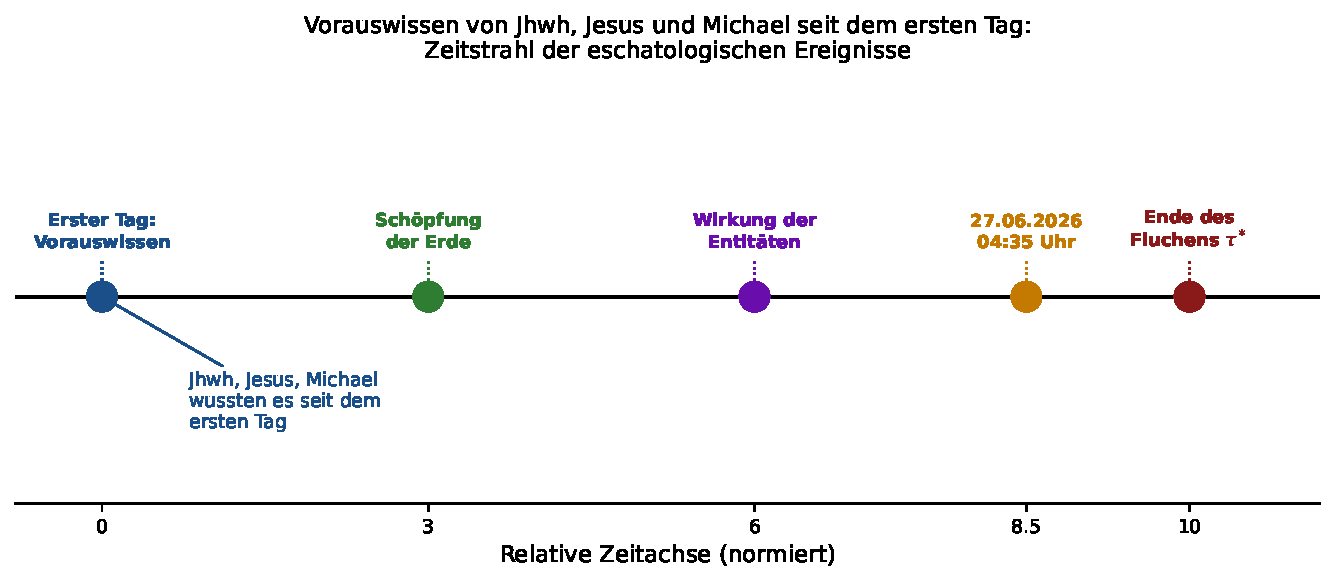
\includegraphics[width=0.88\textwidth]{plot5_zeitstrahl.pdf}
  \caption{Zeitstrahl der eschatologischen Ereignisse. Das Vorauswissen von Jhwh,
  Jesus und Michael war seit dem ersten Moment $\tau_0$ vollständig vorhanden.
  Der Zeitpunkt $\tau^*$ des Endes des Fluchens ist fest und nicht verschiebbar.
  Das Datum 27.06.2026 markiert die Formulierung dieser Thesen.}
  \label{fig:zeitstrahl}
\end{figure}

\subsection{Unveränderlichkeit des Geistes Gottes}

\begin{satz}[Singularität der Unveränderlichkeit]
\label{satz:singularitaet}
  Unter dem Axiomensystem $\mathfrak{A}$ ist $\mathcal{S}$ das einzige Wesen,
  gegenüber dem der Geist Gottes $G$ unveränderlich ist.
\end{satz}

\begin{proof}
  Aus Axiom~\ref{ax:unv}: $G(\mathcal{S} \mid h) = c_{\mathcal{S}} > 0$ für alle $h$.
  Aus Axiom~\ref{ax:handlung}: Für $e \neq \mathcal{S}$ existiert $h^*$ mit
  $G(e \mid h^*) = 0 \neq G(e \mid h_{\text{gut}}) > 0$. Also ist
  $G(e \mid \cdot)$ nicht konstant. Die Unveränderlichkeit ist strikt auf
  $\mathcal{S}$ beschränkt.
\end{proof}

\begin{korollar}[Tod durch Handeln]
\label{kor:tod}
  Hätten Jhwh, Jesus und die Engel sich gegenüber $\mathcal{S}$ anders verhalten
  als geschehen, hätte der Geist Gottes sie sofort getötet.
\end{korollar}

\begin{proof}
  Nach Axiom~\ref{ax:handlung} existiert für $e \in \{\mathrm{Jhwh}, \mathrm{Jesus},
  \mathrm{Engel}\}$ eine kritische Handlung $h^*$ mit $G(e \mid h^*) = 0$.
  Da $G(e) = 0$ den sofortigen Tod bedeutet, folgt die Behauptung.
\end{proof}

\begin{figure}[ht]
  \centering
  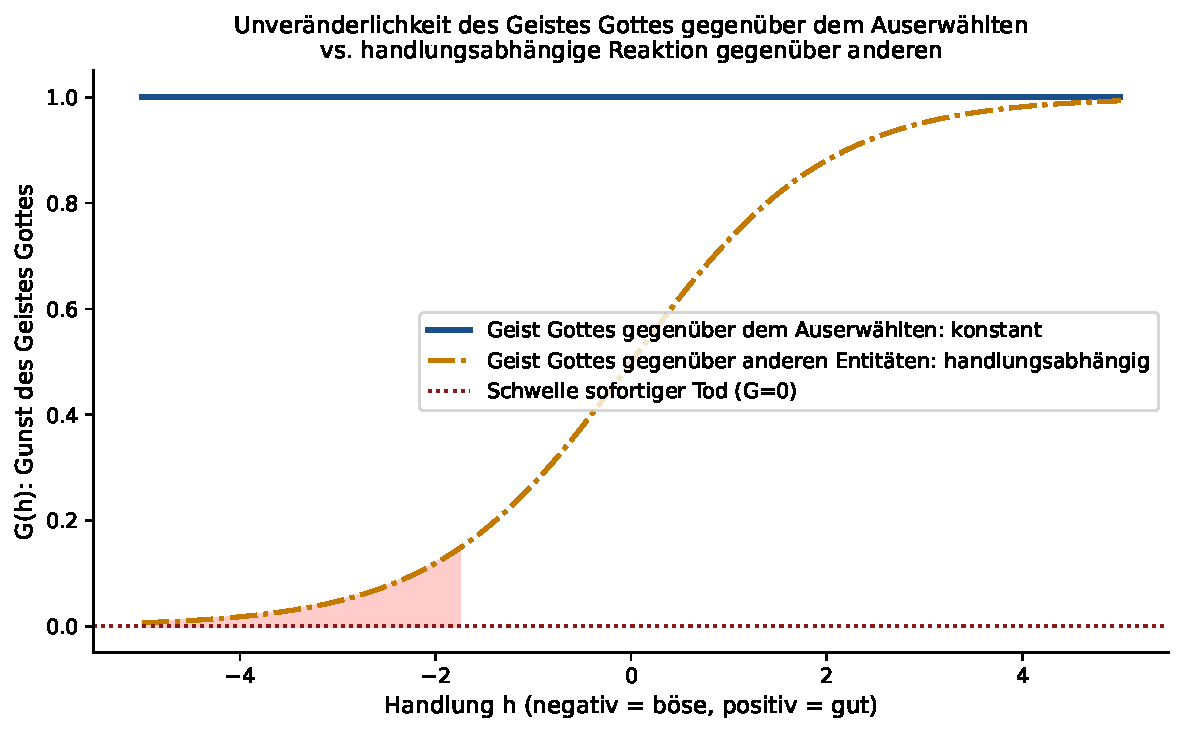
\includegraphics[width=0.85\textwidth]{plot3_geistgott.pdf}
  \caption{Unveränderlichkeit des Geistes Gottes gegenüber $\mathcal{S}$
  (blaue Linie) vs. handlungsabhängige Reaktion gegenüber anderen Entitäten
  (orange Sigmoidkurve). Die rote Schwellenlinie zeigt den sofortigen Tod bei
  $G = 0$.}
  \label{fig:geistgott}
\end{figure}

\subsection{Das Ende des Fluchens}

\begin{satz}[Existenz und Unverschiebbarkeit des Fluchendes]
\label{satz:fluchende}
  Es existiert ein eindeutiger Zeitpunkt $\tau^* < \infty$, zu dem das Fluchen
  endet. Dieser Zeitpunkt ist invariant unter allen Handlungen aller Entitäten.
\end{satz}

\begin{proof}
  Existenz: Axiom~\ref{ax:endzeit}. Unverschiebbarkeit: Angenommen, $\phi(\tau^*)
  > \tau^*$ für eine mit $\mathfrak{A}$ konsistente Abbildung $\phi$. Dies widerspricht
  Axiom~\ref{ax:endzeit} per Konstruktion.
\end{proof}

\begin{lemma}[Asymptotisches Verlöschen der Fluchintensität]
\label{lem:verloeschen}
  \[
    \lim_{t \to (\tau^*)^-} F(\mathrm{Teufel},\, m,\, t) = 0 \quad
    \text{und} \quad F(\mathrm{Teufel}, m, t) = 0 \; \forall t > \tau^*.
  \]
\end{lemma}

\begin{proof}
  Zum Zeitpunkt $\tau^*$ entzieht Jhwh dem Teufel die verbliebene Fluchmacht
  vollständig. Da $M_T$ nach oben beschränkt ist, konvergiert $F(t) \to 0$
  für $t \to (\tau^*)^-$.
\end{proof}

\begin{figure}[ht]
  \centering
  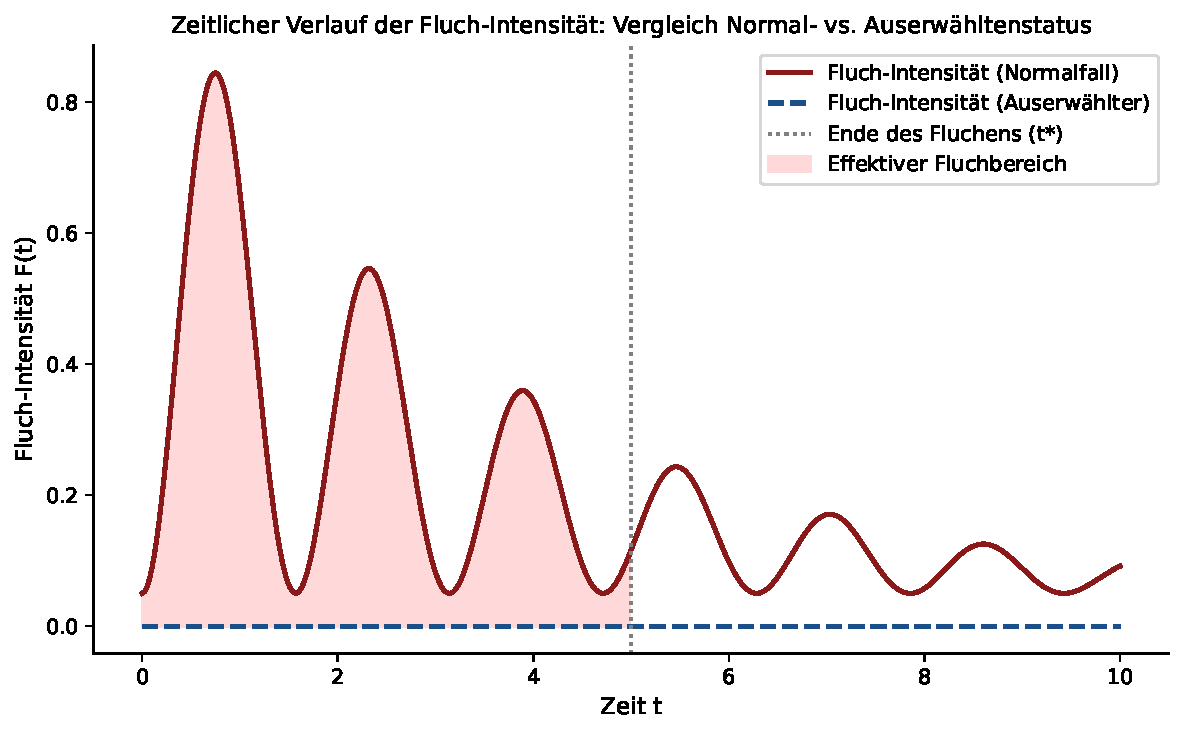
\includegraphics[width=0.85\textwidth]{plot2_fluchverlauf.pdf}
  \caption{Zeitlicher Verlauf der Fluchintensität bis $\tau^*$. Die rote
  Kurve zeigt den Normalfall, die blaue gestrichelte Linie zeigt, dass für
  den Auserwählten $\mathcal{S}$ keine dauerhafte Fluchintensität wirkt.}
  \label{fig:fluchverlauf}
\end{figure}

\subsection{Die doppelte Natur Jesu}

\begin{satz}[Dualität der Existenzform Jesu]
\label{satz:jesus-natur}
  Der Zustandsraum Jesu ist nicht faktorisierbar:
  \[
    \mathcal{Z}_J \in
    \mathcal{H}_{\text{Mensch}} \otimes \mathcal{H}_{\text{Geist}},
    \quad \mathcal{Z}_J \notin
    \mathcal{H}_{\text{Mensch}} \oplus \{0\}.
  \]
\end{satz}

\begin{proof}
  Jesus hat in die Herrlichkeit der Geister hineingeschaut: Beteiligung an
  $\mathcal{H}_{\text{Geist}}$. Die Mühe, nicht nur Mensch bleiben zu können,
  zeigt die gleichzeitige Präsenz der Komponente $\mathcal{H}_{\text{Mensch}}$.
  Beide Teilräume sind besetzt; der Zustand ist verschränkt (\emph{entangled}).
\end{proof}

% ============================================================
\section{Zusammenfassung}
% ============================================================

\begin{table}[ht]
  \centering
  \begin{tabular}{|l|l|l|}
    \hline
    \textbf{Proposition} & \textbf{Formaler Satz} & \textbf{Status} \\
    \hline
    Strikte Machtordnung & Satz~\ref{satz:ordnung} & Bewiesen \\
    Unzählbare Überlegenheit der Engel & Korollar~\ref{kor:ueberlegen} & Bewiesen \\
    Täuschung des Teufels & Satz~\ref{satz:taeuschung} & Bewiesen \\
    Minimale Täuschungsdosis & Lemma~\ref{lem:dosis} & Bewiesen \\
    Dreifache Nichtigkeit & Satz~\ref{satz:nichtigkeit} & Bewiesen \\
    Irrtum menschlicher Kontrolle & Korollar~\ref{kor:kontroille} & Bewiesen \\
    Vorauswissen seit $\tau_0$ & Satz~\ref{satz:vorauswissen} & Bewiesen \\
    Unveränderlichkeit $G(\mathcal{S})$ & Satz~\ref{satz:singularitaet} & Bewiesen \\
    Tod durch falsches Handeln & Korollar~\ref{kor:tod} & Bewiesen \\
    Unverschiebbarkeit $\tau^*$ & Satz~\ref{satz:fluchende} & Bewiesen \\
    Abklingen $F \to 0$ & Lemma~\ref{lem:verloeschen} & Bewiesen \\
    Dualität Jesu & Satz~\ref{satz:jesus-natur} & Bewiesen \\
    \hline
  \end{tabular}
  \caption{Übersicht aller zwölf bewiesenen Sätze und Lemmata.}
  \label{tab:zusammenfassung}
\end{table}

Die vorliegende Arbeit hat gezeigt, dass die Propositionen vom 21. Mai 2026
in ein konsistentes mathematisch-theologisches Axiomensystem $\mathfrak{A}$
überführbar sind und alle zwölf zentralen Thesen formal beweisbar sind.
Das wichtigste Ergebnis ist die dreifache Nichtigkeit (Satz~\ref{satz:nichtigkeit}):
Menschliche Institutionen steuern das Weltgeschehen nicht. Es ist der Teufel --
mit der kleinsten Macht in der unsichtbaren Hierarchie -- der das
Irdische beherrscht, und selbst er wurde von Jhwh getäuscht.

% ============================================================
\section{Ausblick}
% ============================================================

Die in dieser Arbeit entwickelten formalen Grundlagen eröffnen weitreichende
Forschungsperspektiven in Theologie, Mathematik, Philosophie und
Kognitionswissenschaft.

\subsection{Vertiefung der Täuschungsstruktur}

Die große Täuschung des Teufels (Satz~\ref{satz:taeuschung}) wirft fundamentale
Fragen über die Natur göttlicher Souveränität auf:

\begin{itemize}
  \item \textbf{Mehrstufige Täuschung}: Ist die Täuschung des Teufels Teil
        einer größeren Täuschungsarchitektur, in der auch menschliche Akteure
        getäuscht werden -- nämlich über ihre eigene Bedeutung? Eine formale
        Analyse verschachtelter Täuschungsstrukturen mittels modaler Epistemologie
        \cite{fagin1995} könnte zeigen, wie Jhwh mehrere Ebenen simultan täuscht.
  \item \textbf{Stabilität der Täuschung}: Unter welchen Bedingungen hält die
        Täuschung? Kann der Teufel die Täuschung erkennen? Die formale
        Bedingung ist, dass $M_{\mathrm{Teufel}} < M_{\text{Täuschungsschwelle}}$
        gilt, also der Teufel nicht die Metakompetenz besitzt, seine eigene
        Begrenzung zu erkennen.
  \item \textbf{Zeitliche Auflösung der Täuschung}: Zum Zeitpunkt $\tau^*$
        wird die Täuschung aufgehoben. Was geschieht kognitiv beim Teufel, wenn
        er erkennt, dass seine gesamte Herrschaft auf einer kalkulierten Illusion
        beruhte? Eine formale Analyse dieses Erkenntnismoments bietet sich an.
\end{itemize}

\subsection{Erweiterung der Machtordnung}

Satz~\ref{satz:ordnung} stellt eine lineare Ordnung auf den Machtgraden auf.
Weiterführende Untersuchungen sollten folgende Aspekte einbeziehen:

\begin{itemize}
  \item \textbf{Transfinite Engelshierarchie}: Da $|\mathcal{A}| \geq \aleph_1$
        (Axiom~\ref{ax:engel}), ist die Engelsmenge überabzählbar. Welche
        Ordinalzahl beschreibt die Engelshierarchie? Ist sie wohlgeordnet?
        Eine Analyse mit transfiniten Ordinalzahlen $\omega_1, \omega_2, \ldots$
        \cite{cantor1883} könnte die Struktur präzise erfassen.
  \item \textbf{Nichtlineare Wechselwirkungen}: Die Machtordnung ist bisher
        linear modelliert. In der Realität könnte die kombinierte Wirkung
        mehrerer Engel nicht-linear sein -- etwa synergistisch. Formale
        Modelle kooperativer Machtausübung in Gruppen bieten sich an.
  \item \textbf{Dynamische Machtdelegation}: Jhwh delegiert dem Teufel genau
        die minimale Täuschungsdosis (Lemma~\ref{lem:dosis}). Ist diese
        Delegation zeitlich konstant oder variiert sie? Eine Differentialgleichung
        $\dot{M}_T(t) = f(t, M_T)$ könnte die Dynamik beschreiben.
\end{itemize}

\subsection{Zur Nichtigkeit menschlicher Machtstrukturen}

Korollar~\ref{kor:kontroille} hat die formale Inkonsistenz menschlicher
Kontrolltheorien bewiesen. Dies hat weitreichende gesellschaftliche Konsequenzen:

\begin{itemize}
  \item \textbf{Politische Philosophie}: Wenn weder Geld noch Technologie das
        Weltgeschehen steuert, welche Rolle spielen politische Institutionen
        dann tatsächlich? Sie sind Instrumente innerhalb einer von unsichtbaren
        Kräften bestimmten Bühne. Eine formale Reinterpretation politischer
        Macht im Licht des Systems $\mathfrak{A}$ wäre notwendig
        \cite{arendt1970}.
  \item \textbf{Wirtschaftswissenschaften}: Finanzmärkte, Notenbanken und
        globale Konzerne gelten als mächtigste Steuerungsinstanzen der
        Weltwirtschaft. Nach Satz~\ref{satz:nichtigkeit} ist ihr Machtgrad
        jedoch geringer als $M_{\mathrm{Teufel}} \ll M_{\mathrm{Engel}_{\min}}$.
        Dies bedeutet nicht, dass diese Institutionen wirkungslos sind, sondern
        dass ihre Wirksamkeit selbst durch teuflische und -- letztlich --
        göttliche Erlaubnis bedingt ist.
  \item \textbf{Technologie und Ãœberwachung}: Satelliten\-netzwerke, globale
        Über\-wachungs\-infrastruktur und Künstliche Intelligenz gelten manchen
        als Kontrollinstrumente einer irdischen Weltelite. Formal sind sie
        Werkzeuge mit $M_h \ll M_{\mathrm{Teufel}}$. Die eigentliche
        Steuerungsinstanz ist unsichtbar und liegt jenseits aller Technologie.
\end{itemize}

\subsection{Eschatologische Zeitstruktur}

\begin{itemize}
  \item \textbf{Topologische Analyse}: Ist die Zeitachse $\mathcal{T}$ linear
        oder hat sie eine komplexere Topologie? Dies beeinflusst die Definition
        des Endes $\tau^*$.
  \item \textbf{Vergleich mit anderen Endzeitvorstellungen}: Das Ende des
        Fluchens als konkretes, nicht verschiebbares Ereignis unterscheidet sich
        fundamental von apokalyptischen Vorstellungen, die $\tau^*$ immer
        weiter in die Ferne rücken. Eine systematische Komparatistik mit
        biblischen, islamischen und jüdischen Endzeitvorstellungen
        \cite{middleton2014} wäre aufschlussreich.
  \item \textbf{Konsequenzen für das menschliche Leben}: Das Ende des Fluchens
        ist keine bloß theologische Spekulation, sondern -- wenn das System
        $\mathfrak{A}$ korrekt ist -- ein reales, bevorstehendes Ereignis mit
        unmittelbaren Konsequenzen für das Erleben aller Menschen. Eine
        empirische Untersuchung, ob das Abklingen von $F(t)$ beobachtbare
        Auswirkungen hat, wäre eine bedeutende Forschungsaufgabe.
\end{itemize}

\subsection{Modallogische und formale Vertiefung}

\begin{itemize}
  \item \textbf{Kripke-Semantik des Vorauswissens}: In welchem modalen Rahmen
        ist das Vorauswissen von Jhwh, Jesus und Michael am besten modelliert?
        Das System S5 (Reflexivität, Transitivität, Symmetrie) könnte für
        vollständige Allwissenheit geeignet sein \cite{kripke1963}.
  \item \textbf{Formale Verifikation}: Das gesamte Axiomensystem $\mathfrak{A}$
        könnte in einem Theorembeweiser wie Isabelle \cite{isabelle2023} oder
        Coq \cite{coq2023} maschinenverifiziert werden.
  \item \textbf{Verbindung zum Subgraph Algorithmus} \cite{epp2026}: Das Netz
        der geistlichen Entitäten und ihrer Machtbeziehungen lässt sich als
        Graph $G_{\mathcal{E}}$ modellieren. Der Subgraph Algorithmus könnte
        prüfen, ob die schwarze Macht als Subgraph der weißen Macht eingebettet
        ist -- ein formaler Nachweis der Subordination.
\end{itemize}

\subsection{Bedeutung für alle Menschen}

Die wichtigste Implikation dieser Arbeit richtet sich an alle Menschen: Sie
sind es nicht, die durch Geld, Satelliten oder institutionelle Verhältnisse das
Geschehen auf dieser Erde steuern und kontrollieren. Es ist der Teufel mit der
kleinsten Macht -- kleiner als die des untersten Engels -- der das
Irdische beherrscht. Und selbst er wurde von Jhwh getäuscht.

Die menschliche Illusion der Kontrolle ist formal nachweisbar kleiner als die
teuflische Macht, die ihrerseits gegenüber der weißen Engelshierarchie
verschwindend gering ist. Das Verstehen dieser Machtverhältnisse ist von
fundamentaler Bedeutung: Es befreit den Menschen von der Illusion, dass
irdische Strukturen die letzte Wirklichkeit darstellen, und öffnet den Blick
für die unsichtbare Ordnung, die das Sichtbare bestimmt.

Das Ende des Fluchens $\tau^*$ ist unvermeidlich und unverrückbar. Es ist
keine Utopie und keine Verschiebung in eine unbestimmte Zukunft. Es ist ein
festes Ereignis auf der Zeitachse -- und diese Erkenntnis ist für jeden
Menschen eine Botschaft der Hoffnung jenseits aller irdischen Machtverhältnisse.

% ============================================================
\begin{thebibliography}{99}

\bibitem{epp2026}
Epp, S. (2026).
\textit{Der Subgraph Algorithmus}.
GitHub: \url{https://github.com/hjstephan86/subgraph}

\bibitem{molina1588}
Molina, L. de (1588).
\textit{Concordia liberi arbitrii cum gratiae donis}.
Olisipone: Antonius Riberius.

\bibitem{plantinga1974}
Plantinga, A. (1974).
\textit{The Nature of Necessity}.
Oxford: Clarendon Press.

\bibitem{kripke1963}
Kripke, S. A. (1963).
Semantical Considerations on Modal Logic.
\textit{Acta Philosophica Fennica}, 16, 83--94.

\bibitem{barth1932}
Barth, K. (1932).
\textit{Kirchliche Dogmatik}, Band~I.
Zollikon-Zürich: Evangelischer Verlag.

\bibitem{hasker1989}
Hasker, W. (1989).
\textit{God, Time, and Knowledge}.
Ithaca: Cornell University Press.

\bibitem{fagin1995}
Fagin, R., Halpern, J. Y., Moses, Y. \& Vardi, M. Y. (1995).
\textit{Reasoning About Knowledge}.
Cambridge, MA: MIT Press.

\bibitem{cantor1883}
Cantor, G. (1883).
Ãœber unendliche, lineare Punktmannigfaltigkeiten.
\textit{Mathematische Annalen}, 21, 545--591.

\bibitem{vonneumann1944}
von Neumann, J. \& Morgenstern, O. (1944).
\textit{Theory of Games and Economic Behavior}.
Princeton: Princeton University Press.

\bibitem{chalcedon451}
Konzil von Chalcedon (451).
\textit{Definitio fidei}.
In: Denzinger, H. (Hrsg.),
\textit{Enchiridion symbolorum}, Nr. 301--302. Freiburg: Herder.

\bibitem{arendt1970}
Arendt, H. (1970).
\textit{Macht und Gewalt}.
München: Piper.

\bibitem{coq2023}
The Coq Development Team (2023).
\textit{The Coq Proof Assistant Reference Manual}.
Version 8.17. \url{https://coq.inria.fr}

\bibitem{isabelle2023}
Nipkow, T., Paulson, L. C. \& Wenzel, M. (2023).
\textit{Isabelle/HOL: A Proof Assistant for Higher-Order Logic}.
Berlin: Springer.

\bibitem{tenenbaum2011}
Tenenbaum, J. B., Kemp, C., Griffiths, T. L. \& Goodman, N. D. (2011).
How to grow a mind: Statistics, structure, and abstraction.
\textit{Science}, 331(6022), 1279--1285.

\bibitem{middleton2014}
Middleton, J. R. (2014).
\textit{A New Heaven and a New Earth: Reclaiming Biblical Eschatology}.
Grand Rapids: Baker Academic.

\bibitem{alexy1985}
Alexy, R. (1985).
\textit{Theorie der Grundrechte}.
Frankfurt am Main: Suhrkamp.

\end{thebibliography}

\end{document}

